\documentclass[]{article}
\usepackage{graphicx}
\graphicspath{ {graphs/} }
\usepackage{geometry}
\geometry{a4paper, portrait, margin=1.0in}
\usepackage{gensymb}
\usepackage{booktabs}

%opening
\title{Identification of Direct Cherenkov Pixels using Boosted Decision Trees}
\author{Robert Stein}
\begin{document}

\maketitle

\begin{abstract}
When Cosmic Rays travel through the atmosphere, the primary particle will often emit some Direct Cherenkov light before the much brighter Extended Air Shower is generated. Unlike the broader air shower component of telescope images, all of the Direct Cherenkov light will usually be concentrated in a single pixel. A new method for identifying these Direct Cherenkov pixels was developed, relying on supervised machine learning. A set of Cosmic Ray telescope images were simulated, both with and without the Extended Air Shower background, for use in classifier training. With reference to the background-free telescope images, the Direct Cherenkov pixel in each corresponding full-shower telescope image could be reliably identified. A Boosted Decision Tree to identify these Direct Cherenkov pixels was trained, using data from the full-shower training images. The Boosted Decision Tree performance was then tested on a second set of full-shower telescope images, and compared to existing methods of Direct Cherenkov pixel identification.
\end{abstract}

\section{Introduction}
A Cosmic Ray will often emit Direct Cherenkov (DC) light in the upper atmosphere, before generating an Extended Air Shower (EAS) through interaction with the lower atmosphere. Analysis of the DC light from a shower can indicate primary particle energy, charge and position. It is consequently very useful to measure the quantity and direction of DC light emission, for use in event reconstruction. There are numerous Telescope Arrays which currently image Cherenkov Light emission from Cosmic Rays in the atmosphere, including the HESS, MAGIC and VERITAS Experiments. In these telescope images, the DC light is usually concentrated in a single  \textquoteleft DC pixel'. Identifying this pixel is challenging, because the brighter EAS Cherenkov light background often overlaps with the DC pixel. 

At present, the DC pixel candidate can be identified by applying a number of cuts to pixels in an image, such as those used by the HESS collaboration \cite{hess07}. The variable $Q_{DC} = \frac{Intensity_{N.N.max}}{Intensity}$ is defined as the ratio of the largest neighbouring pixel intensity to the intensity of a given pixel, and from the subset of pixels passing these cuts, the DC candidate is simply the pixel with the smallest $Q_{DC}$. Despite a good degree of accuracy, this method is very inefficient, leaving the majority of events with no DC candidate. An improved method would aim to increase the number of correctly identified events, while still enabling cuts which discriminate well between correctly and incorrectly identified events.

Classifiers provides an alternative method of identification, making use of supervised machine learning to find structure in datasets. To train a classifier, we require a set of training data entries containing several variables, as well as the correct class for each of the entries in the dataset. Once trained, a classifier can be used to predict the class for any such data entry. In this case, the classifier must learn to distinguish between non-DC and DC pixels. 

The CORSIKA package \cite{Heck98} was used to generate Cosmic Ray events, while the sim\textunderscore telarray package  \cite{Bernlohr08} was used to generate corresponding HESS array telescope images.  Simulation with EAS background was used to produce training pixel sets, while corresponding simulation without EAS background was used to determine the true class of each pixel in the training sets. The data was used to train a Boosted Decision Tree (BDT) classifier to identify DC pixels. The data was provided in the form of individual pixel entries, rather than as discrete sets for images or events.

Once trained, the BDT was applied to all pixel entries in a separate \textquoteleft testing' set of simulated telescope images. For each pixel, the BDT assigned a \textquoteleft Signal Probability', $P_{signal}$, indicating the likelihood of the pixel being a DC pixel. For each image, the pixel with the largest $P_{signal}$ was identified as the sole DC pixel candidate. As before, the true class of each pixel was determined from a second EAS-free simulation. Thus, the accuracy of BDT identification for test telescope images was calculated.

\section{Image Simulation}
The full simulation of air showers was performed using the CORSIKA package, with a standard atmospheric profile derived from measurements conducted at the HESS site in Namibia. In total, 2000 training events and a further 2000 testing events were simulated. The simulated particles were $Fe^{56}$, within the Energy Range of $35-135$ TeV and a spectrum $\phi(E) \propto E^{-2.7}$. For each set of simulated event, 4 unique random number seeds were used to generate the shower. An altitude of 1800m was assumed, again corresponding to the HESS site. The simulated zenith angle ranged from $0\degree < \theta < 2 \degree$, while the simulated azimuth angle ranges from $-2\degree < \phi < 2 \degree$. The four smaller HESS-phase-1 telescopes were arranged in a cross along the x/y axis with the larger HESS-phase-2 \textquoteleft CT5' telescope placed at the center. The length of each cross arm was $85m$. The simulated target region of the cores was chosen to be a square centered on CT5, with each 300m-long side bisecting the x/y axis.

To determine the true class of each pixel, a simulation was initially run with an energy cut of 10 PeV on all muons and electrons. Because this cut exceeded the primary particle energy, neither daughter muons and electrons, nor the photons they would have emitted, were simulated. Thus the hadronic Cherenkov Light from the primary particle and daughter fragments, but not the EAS light, was present in the camera image. A second identical \textquoteleft EAS Simulation' was run including the same random seeds, but without the energy cut on muons and electrons. This gave a complete EAS image including identical DC light.

With the sim\textunderscore telarray package, the expected HESS hardware response to each air shower was simulated. Among other things, the program accounts for atmospheric transmission and density, mirror positions, sizes and reflectivities, camera shadowing and triggering, quantum efficiency and pulse responses. For the full-shower image, the night sky background was also simulated by sim\textunderscore telarray. Due to the comprehensive and detailed nature of these hardware simulations, the resultant images can be considered \textquoteleft realistic' camera images.  However, sim\textunderscore telarray introduces various sources of random noise to the simulation, leading to some divergence between the EAS-free and full-shower images.

\begin{figure}
\newgeometry{a4paper, portrait, margin=1.0in}
\centering
\begin{minipage}{0.45\textwidth}
\centering
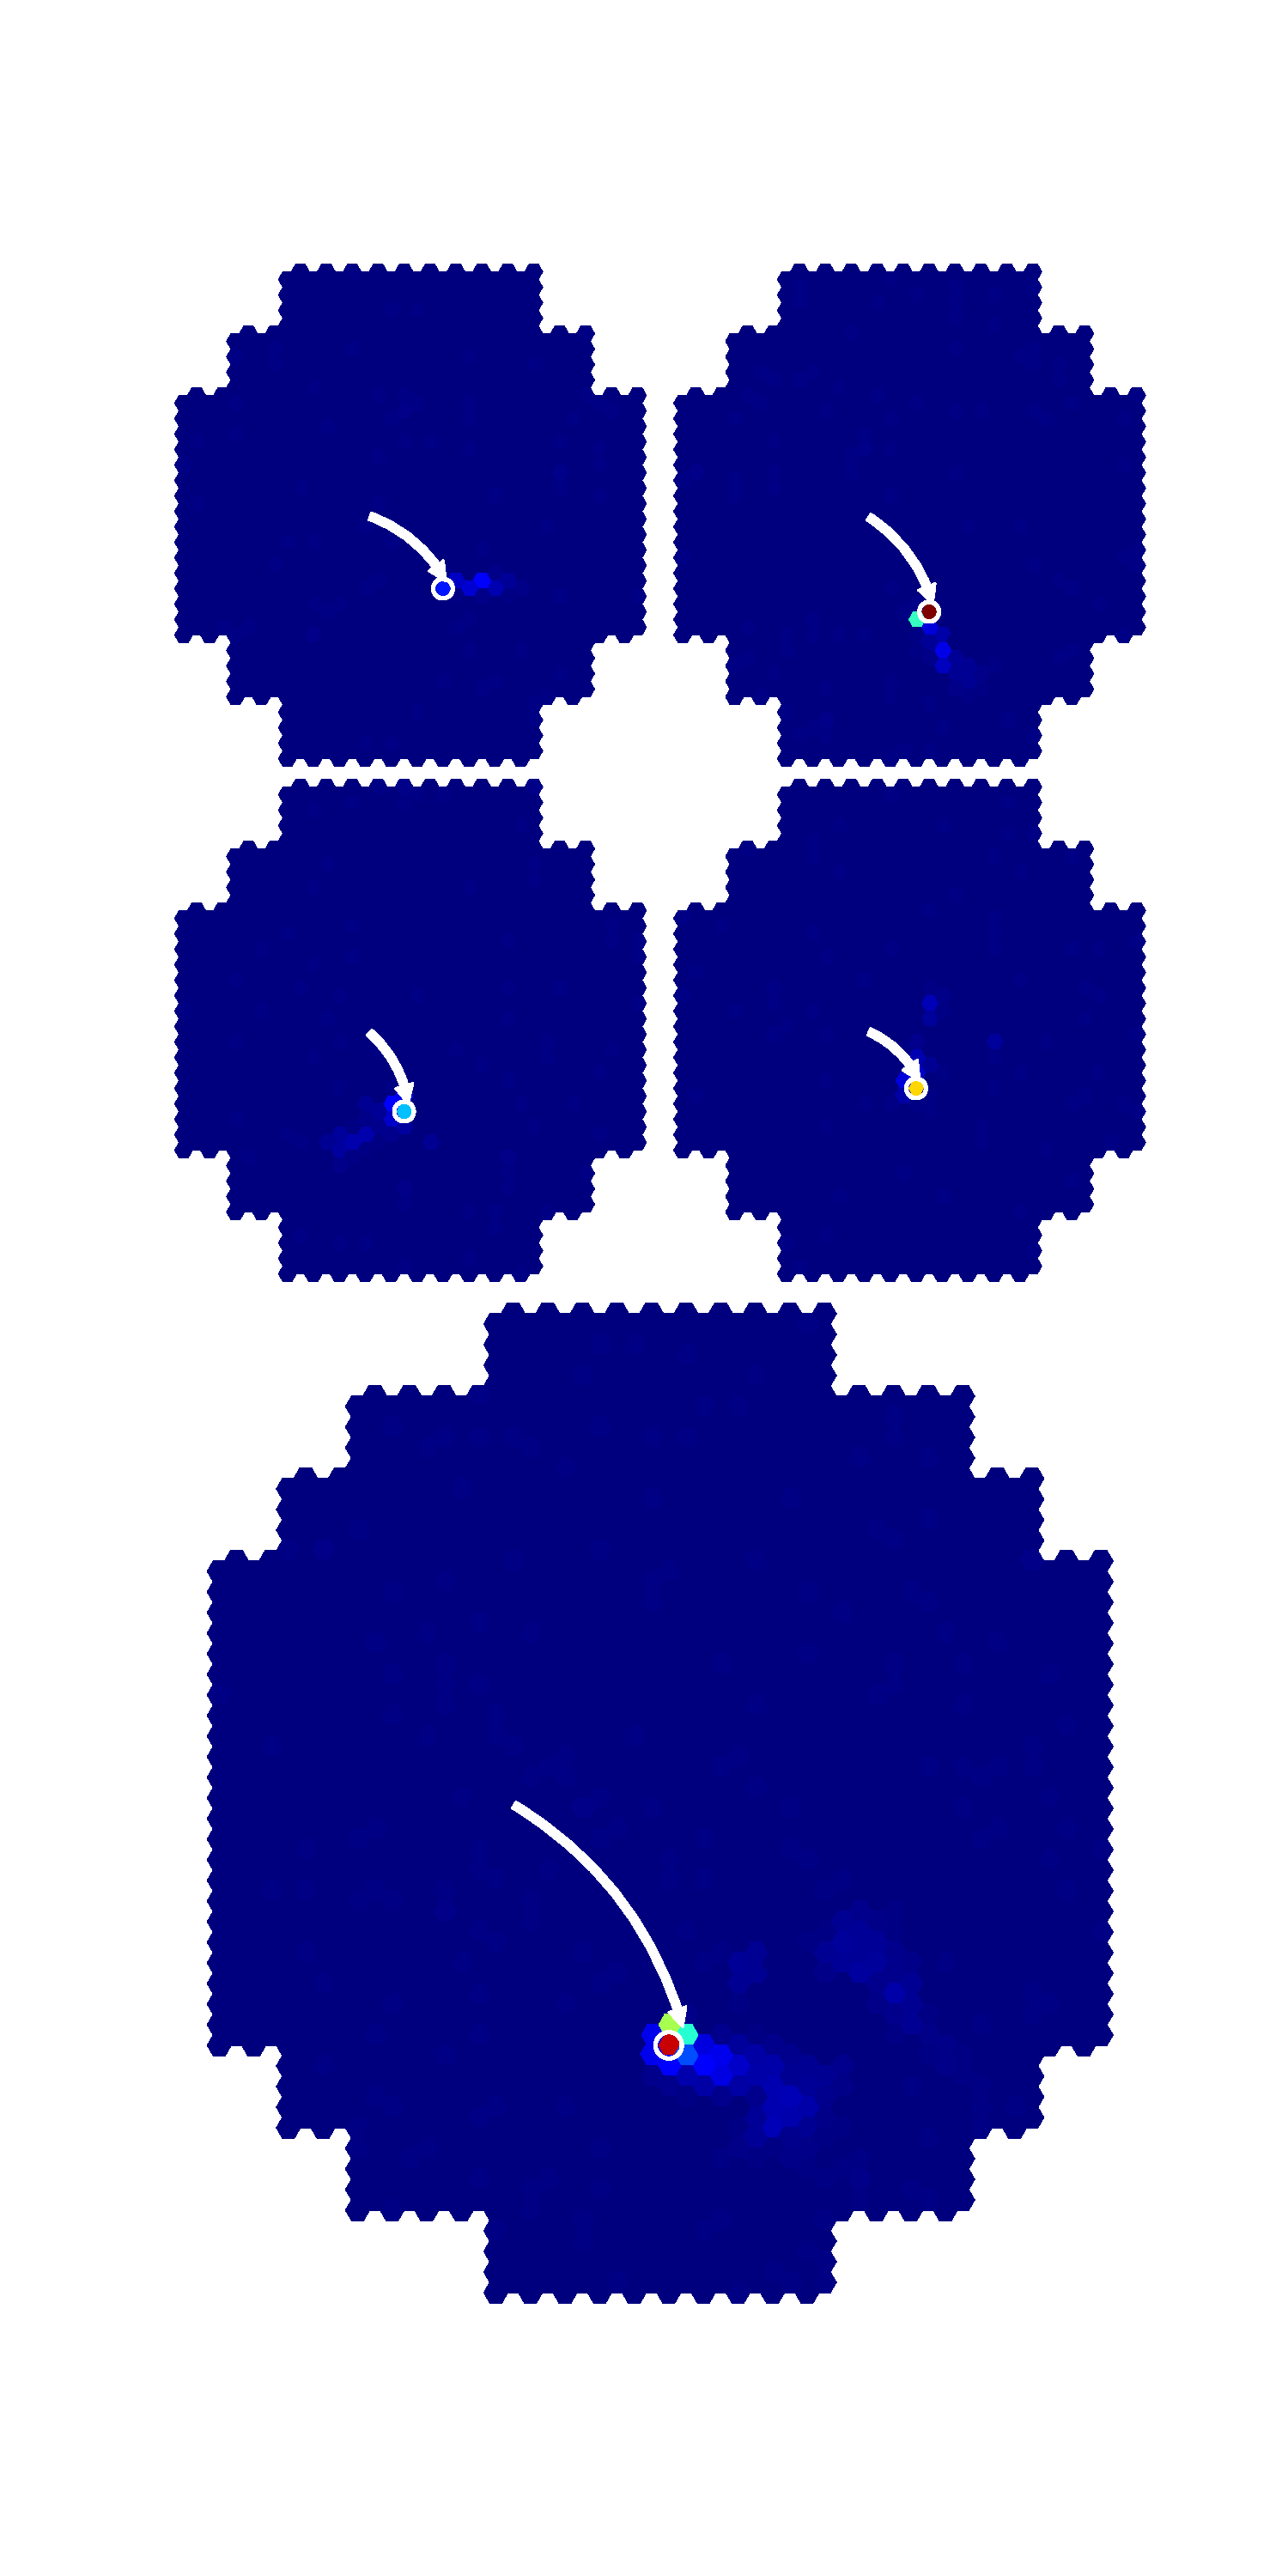
\includegraphics[trim=80 120 80 150,clip,width=\textwidth]{graphDC}
\caption{A typical camera image without the EAS shower. The DC light is visible in every telescope, indicated by the yellow arrow. The shower direction is represented by the white circle. The largest telescope is CT5, but the relative image sizes are not done to scale}
\label{fig:DCtelimage}
\end{minipage}\hfill
\begin{minipage}{0.45\textwidth}
\centering
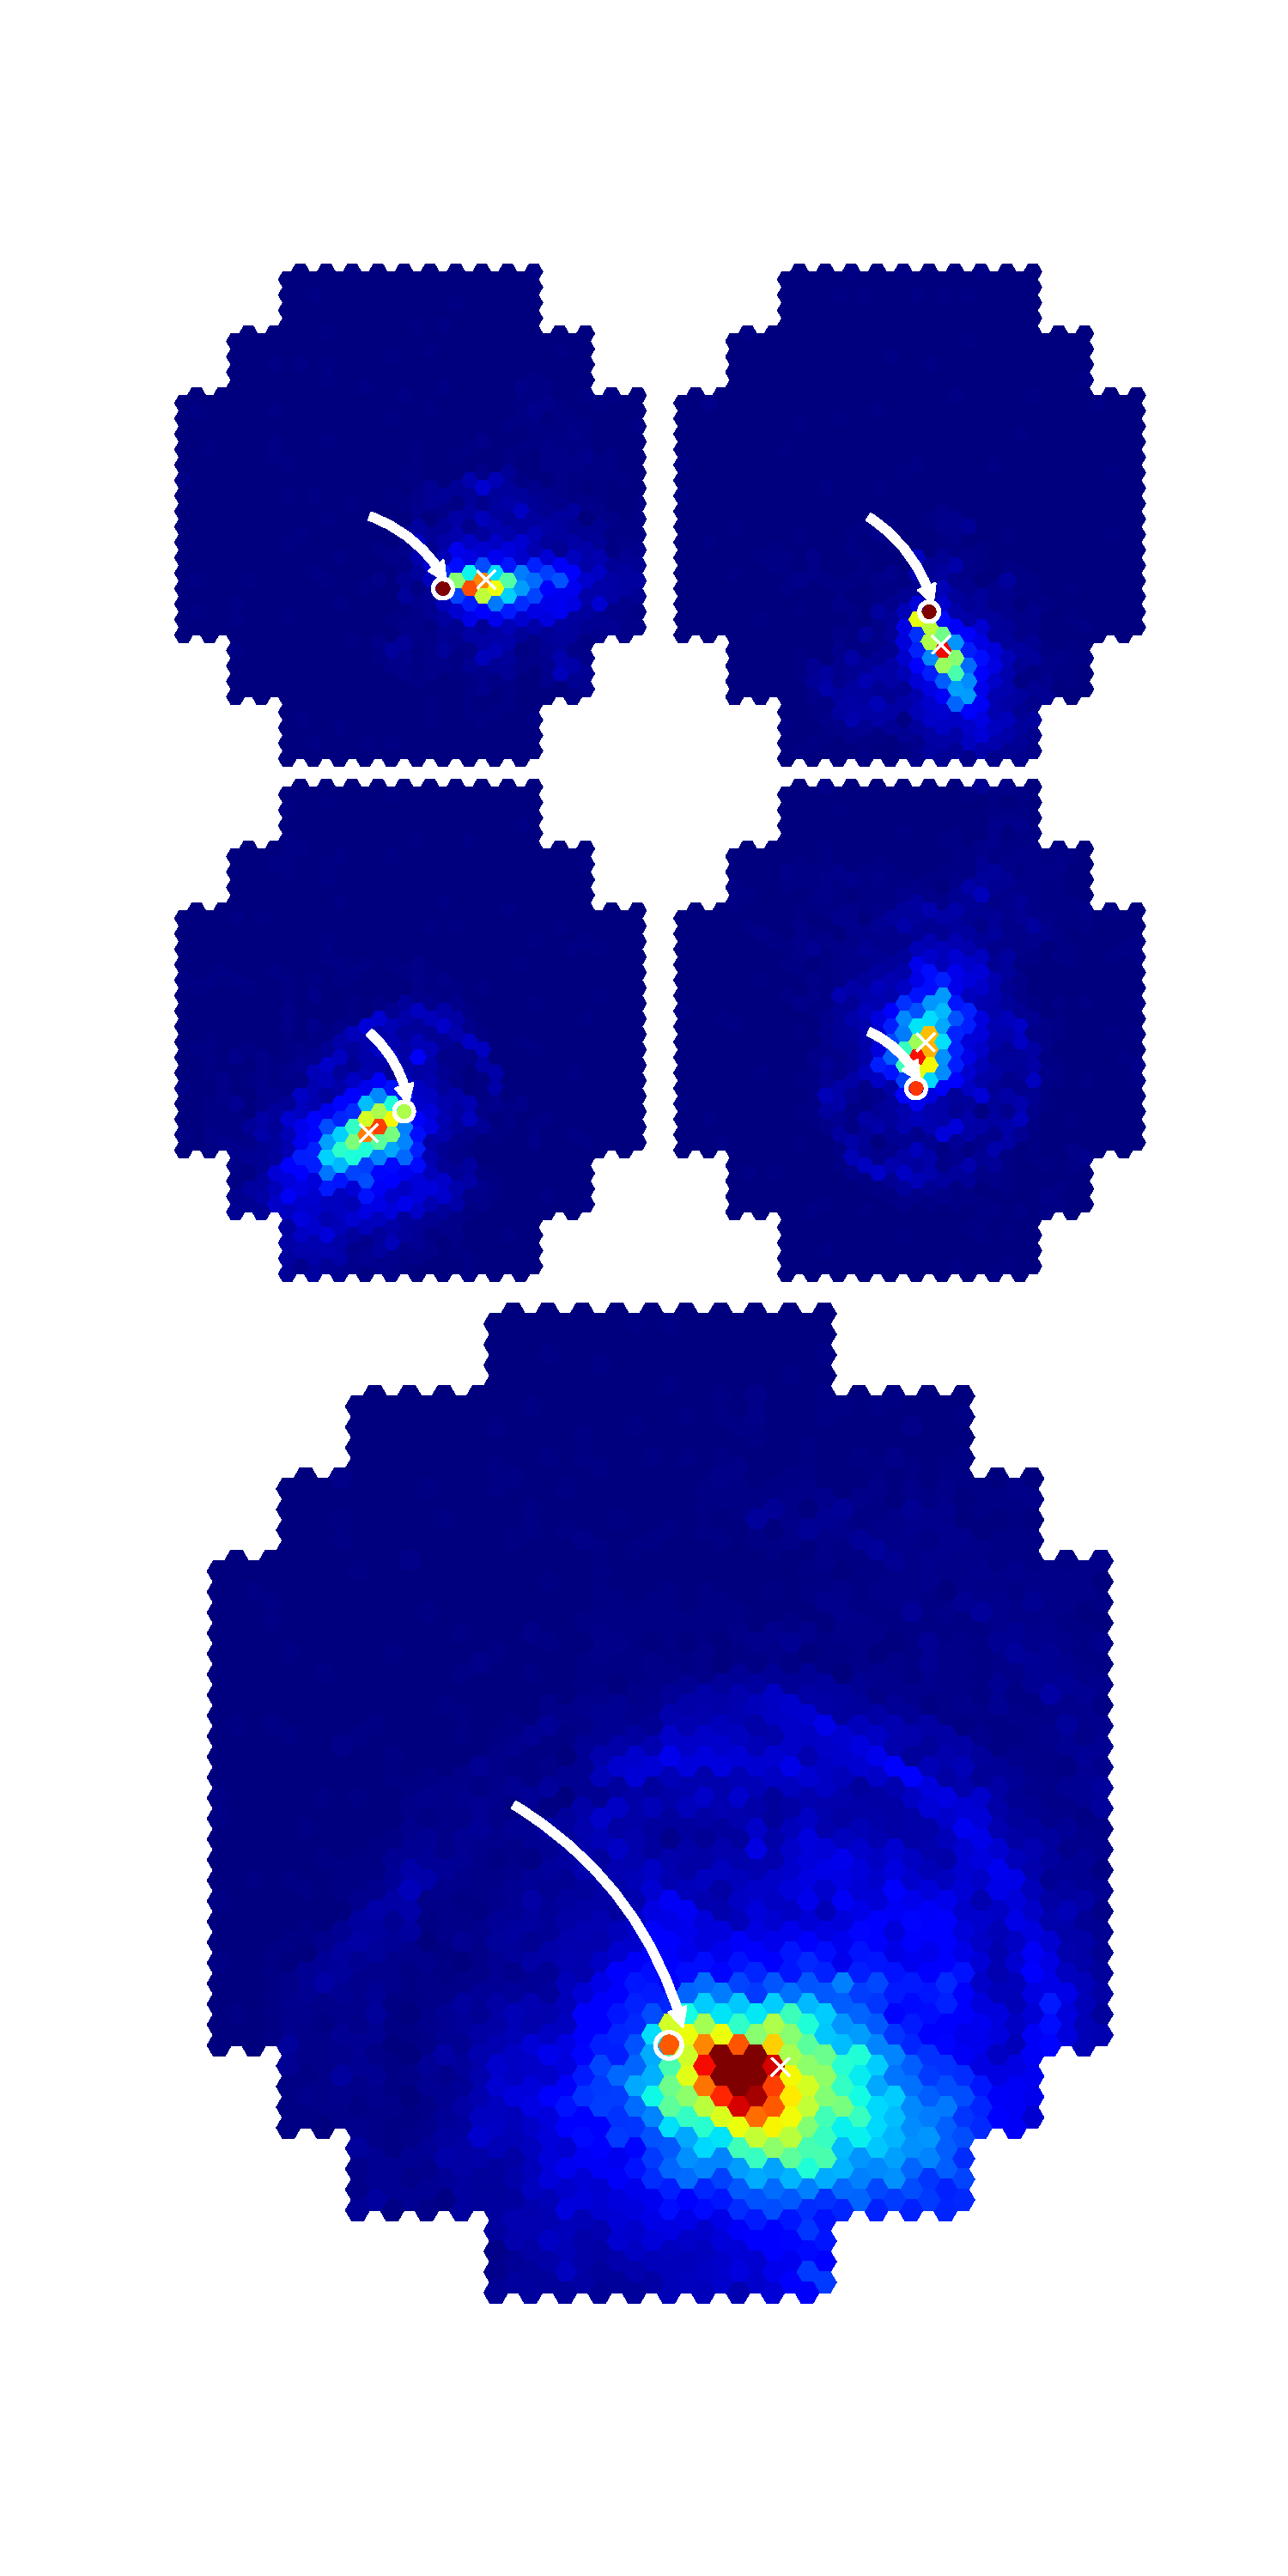
\includegraphics[trim=80 120 80 150,clip,width=\textwidth]{graphfull}
\caption{The same shower as in \ref{fig:DCtelimage} is shown here with the inclusion of the EAS shower. The DC light is pixels are again denoted by an orange circle. The white star represents the BDT-selected DC pixel, while the white cross represents the shower center of gravity.}
\label{fig:cutdistribution2}
\end{minipage}
\restoregeometry
\end{figure}

The various pixel entry variables were then found from the sim\textunderscore telarray output. The HESS telescope pixels have a high gain Channel 0 and a low gain Channel 1, with both voltages undergoing a Flash Analogue-to-Digital Conversion (FADC). The simulated value of the FADC Voltage for each channel was found. Alongside the pedestal and gain, the quantity $Intensity = (FADC - Pedestal)\times Gain $ was calculated. Due to possible saturation of the high gain FADC, only the low gain $Intensity$ was used.

Sim\textunderscore telarray also derives various Hillas whole-image parameters. These include the image width and length measured in degrees, from which the aspect ratio $A.R = \frac{width}{length}$ was calculated. The reconstructed shower direction and the shower center of gravity were also calculated, as positions in azimuth and zenith. Additionally the estimated energy and distance from each telescope to core, $r_{core}$,  were found.

For every pixel, in addition to the $Intensity$, its location within the telescope image was determined using the standard HESS layout. The variables $ \Delta_{C.o.G}$, $\Delta_{Direction}$ and $\Delta_{Line}$ were defined as the distance from the pixel to the shower center of gravity, shower direction, and the line joining those two points. Furthermore, the nearest neigbouring pixel IDs were calculated for every pixel position, enabling the $Intensity$ in each neighbouring pixel to be found. The largest neighbouring intensity was identified, and the ratio $Q_{DC} = \frac{Intensity_{N.N.max}}{Intensity}$ was derived. Similarly the largest neighbouring FADC was found, and the ratio $raw_{Q} = \frac{FADC_{N.N.max}}{FADC}$ was calculated. In addition, the Nearest Neighbour Mean Intensity $Mean_{N.N}$ was recorded. The variable $DC_{Signal} = Intensity-Mean_{N.N}$ was defined as an rough guess of the \textquoteleft DC signal' component in the pixel.

\section{DC Pixel Identification}  
As a basis for comparison, the original HESS cuts listed in \ref{tab:table1} were replicated for the set of test data.   For every image, the total image amplitude $I_{tot}$ was used alongside the zenith angle $\theta$ to determine a unique $Q_{DC}$ cut, reducing the number of accepted DC candidates. For each image, the smallest $Q_{DC}$ among any remaining pixels was used to identify as the DC pixel candidate. Because many images had no pixel that passed all cuts, the $Q_{DC}$ method was frequently unable to identify a DC pixel. In the original analysis, an additional cut $r_{core} \textgreater 40m$ was applied. However, the uncertainty in determining the core position through Hillas Analysis is typically of the order of $\pm 30m$. Consequently, this particular cut was omitted, along with the Impact Parameter cuts. 

\begin{table}[h!]
  \centering
  \caption{Cuts applied to image pixel sets, used by HESS collaboration \cite{hess07}}
  \label{tab:table1}
  \begin{tabular}{ccc}
    \toprule
    Variable & Cut\\
    \midrule
     $ \Delta_{C.o.G}$ & \textgreater 0.17 \\
     $ \Delta_{C.o.G}$ & \textless 0.91 \\
     $\Delta_{Direction}$ & \textless 0.45 \\
     $\Delta_{Line}$ & \textless 0.23 \\
     Aspect Ratio & \textless 0.75 \\
     $Q_{DC}$ & \textless 0.14$ \times \log(\frac{I_{tot}}{161 \times \cos \theta})$ \\
    \bottomrule
  \end{tabular}
\end{table}

The candidates were checked against the true DC pixels identified in the EAS-free images. From the testing sample, 5.2\% of all images were correctly identified and passed the cuts. The $Q_{DC}$ accurate in identifying DC pixels which passed the cuts, as shown in \ref{fig:cutdistribution}. These values served as a benchmark for BDT performance. 

The BDT was trained with the Scikit Learn Python package \cite{scikit-learn}. Using the training set of 2000 CORSIKA events, and randomly split through use of the Python random.random() function into two further subsets, one for learning and one to check overtraining. Within the subset of learning events, every HESS 1 image was used, provided it was triggered in both EAS-free and full-shower simulations. For each of the 1.7 million triggered image pixels, an entry was formed of the variables listed in table \ref{tab:table2}. A class of 0 was assigned to every non-DC pixel, and a class of 1 was assigned to every DC pixel. Having created a dataset, the BDT was then trained with a maximum depth of 8, and 100 trees generated.

\begin{table}[h!]
  \centering
  \caption{Relative Feature Importance in HESS-1 BDT training}
  \label{tab:table2}
  \begin{tabular}{ccc}
    \toprule
    Variable & Relative Importance\\
    \midrule
    $DC_{Count}$ & 0.38\\
    $Mean_{N.N}$ & 0.22\\
    $\Delta_{Direction}$ & 0.15\\
    $Q_{DC}$ & 0.11\\
    $raw_{Q}$ & 0.06\\
    $\Delta_{Line}$ & 0.04\\
    $Intensity$ & 0.04\\
    \bottomrule
  \end{tabular}
\end{table}

The relative importance of each \textquoteleft feature' is automatically calculated by the Scikit Learn package, and is also recorded in table \ref{tab:table2}. The variable $DC_{Count}$ was consistently the most importance variable across many combinations of included variables and BDT training parameters. It was found that, under the conditions listed above, the BDT was 99.94 \% accurate for the entire learning pixel set, and 99.93 \%  accurate for the overtraining-check pixel set. This indicates that the BDT was not significantly overtrained, which would otherwise be manifested by a large divergence in accuracy between learning and overtraining-check data.

Having trained the BDT successfully, it was then applied to the same test dataset as for the classic QDC identification. In each camera image, the event with the largest BDT score was deemed to be \textquoteleft most signal-like', and thus selected as the DC pixel candidate. A cut was applied, requiring $P_{signal} > 0.5$ for the DC candidate to be accepted. A second cut requiring $DC_{Count} > 150$ removed many incorrectly identified events. 

Application of this combined cut greatly increases the successful identification rate. From the testing sample, 37.8\% of all images were correctly identified and passed the cuts. The BDT was found to be 86.0\% accurate in identifying DC pixels which passed the cuts. This represents a very significant improvement in pixel identification efficiency, at the cost of a negligible decrease in accuracy after cuts.

\begin{figure}
\begin{center}
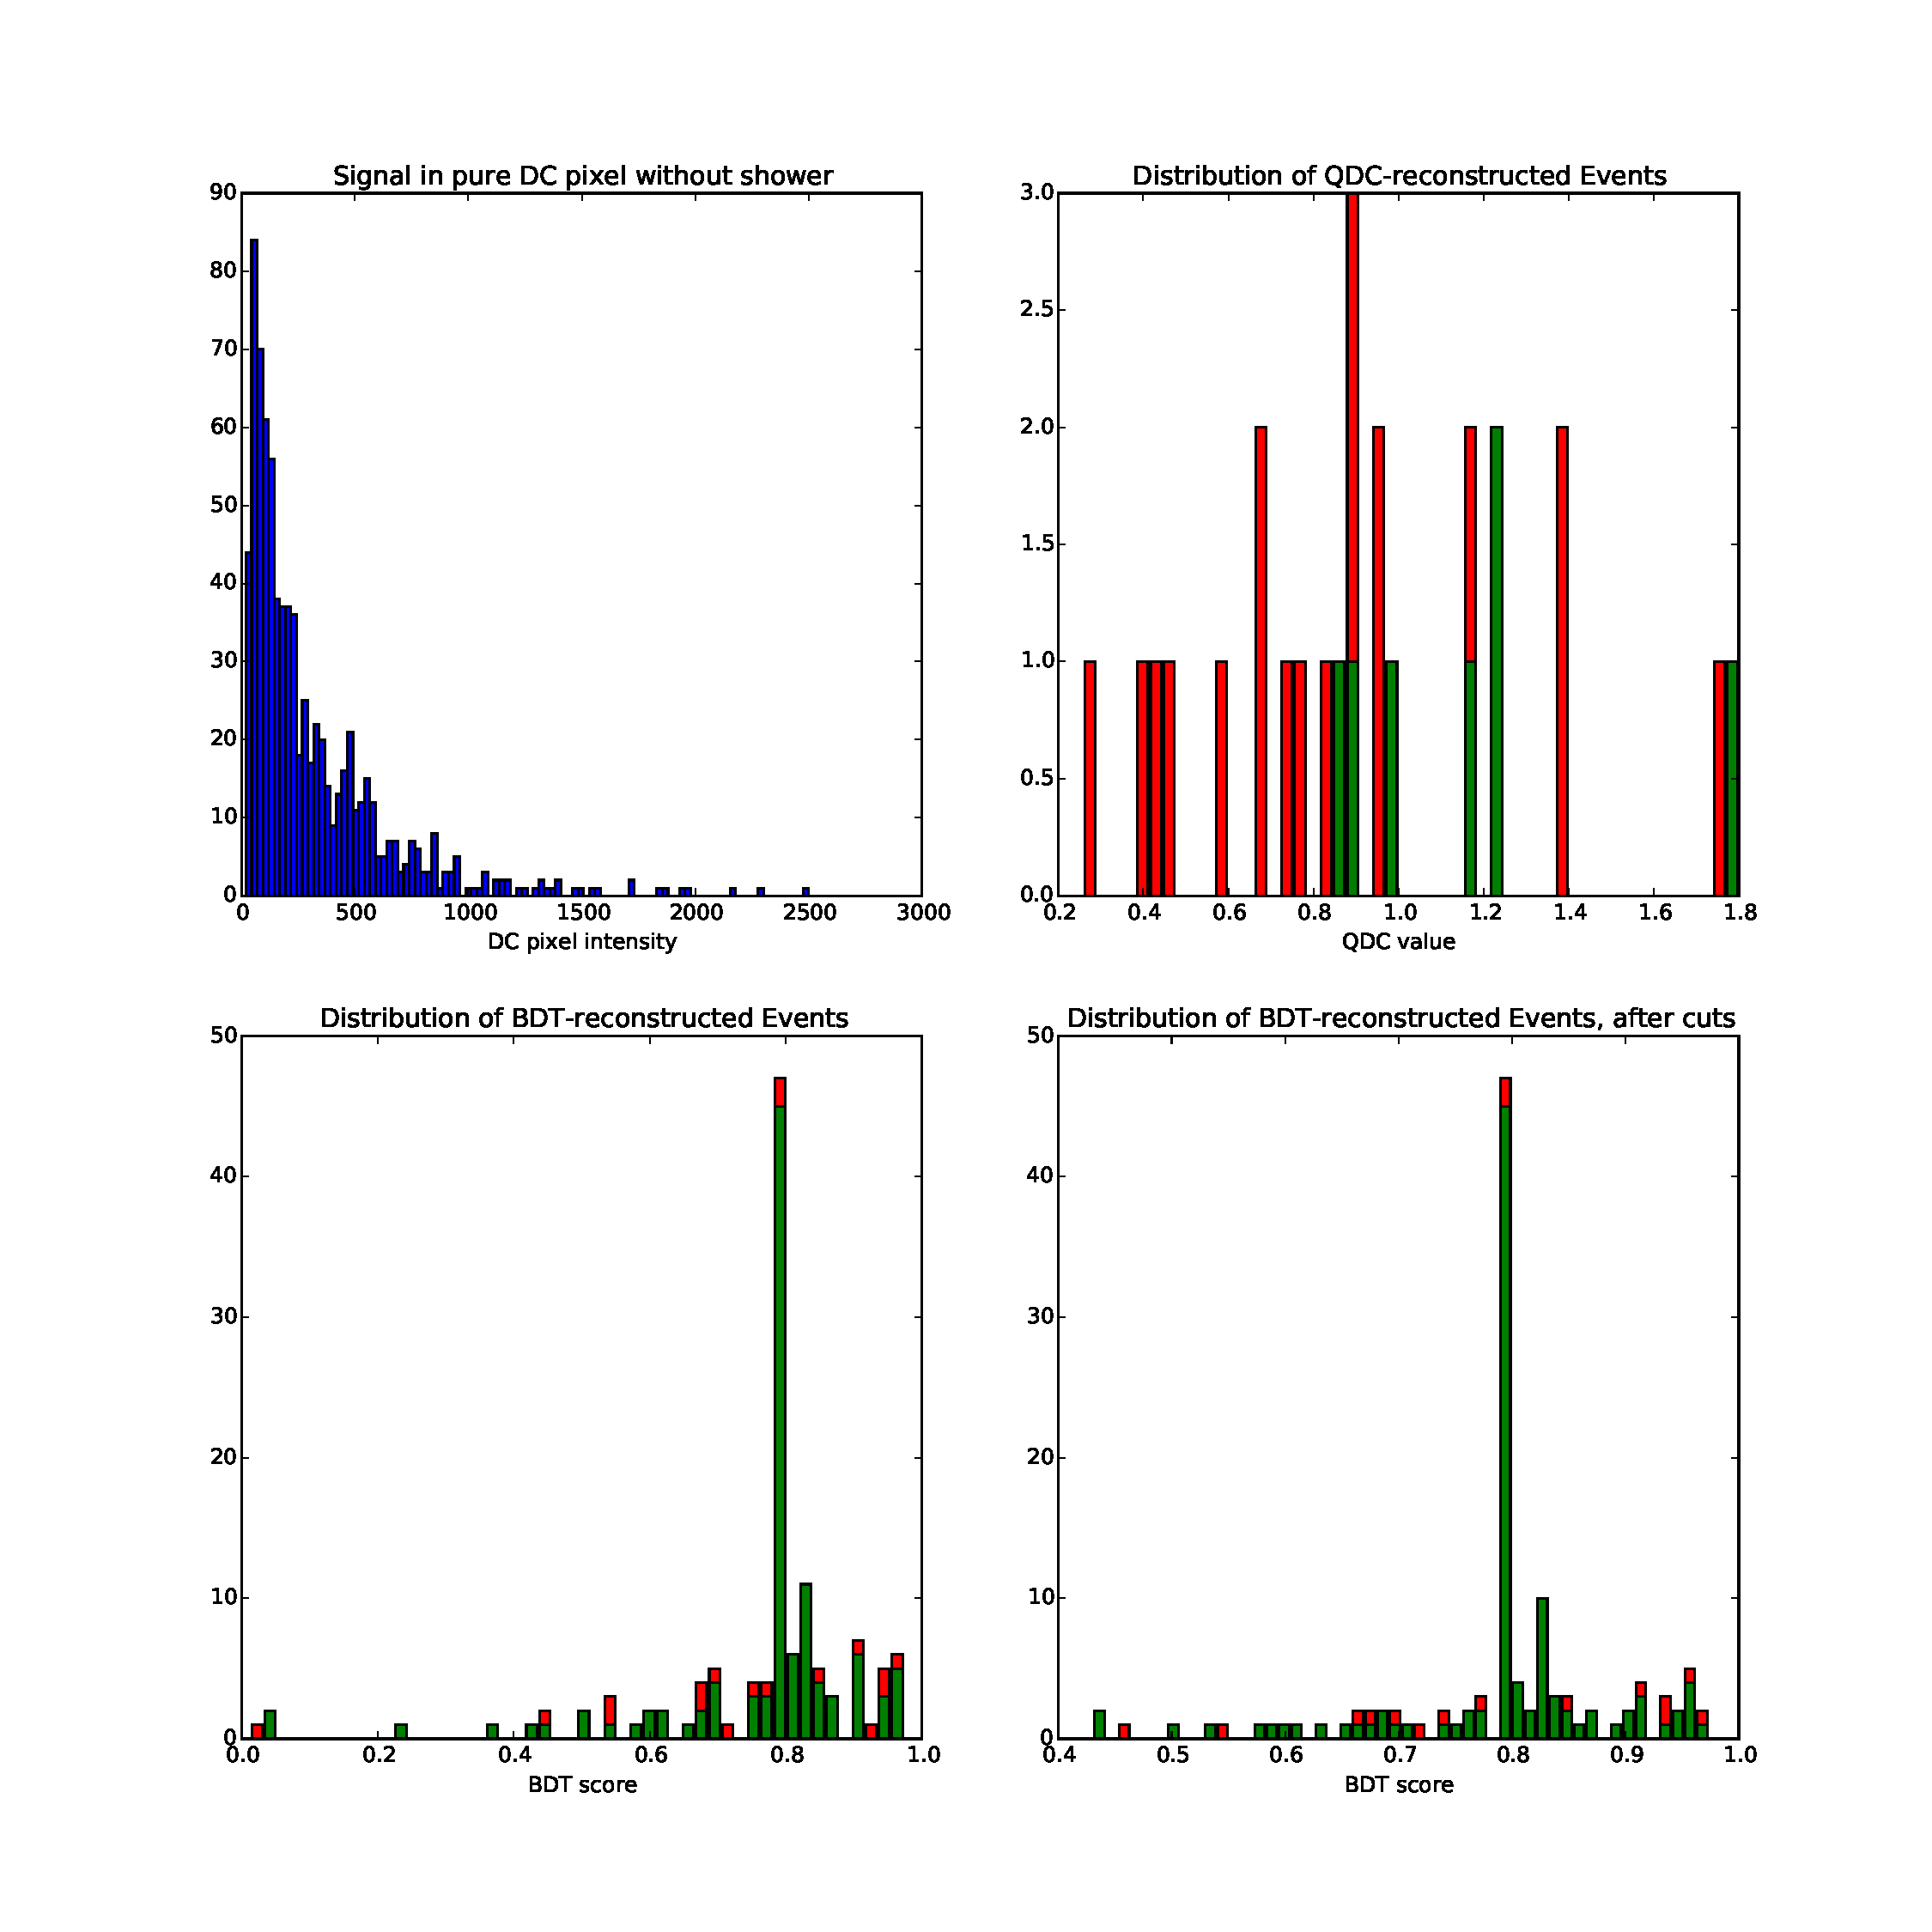
\includegraphics[width=\textwidth]{cutdistribution1None}
\caption{The true $Intensity_{DC}$ in the EAS-free image is shown in the top left, with a broad exponential decay in count as DC intensity increases. Sim\textunderscore telarray requires a minimum of 20 photoelectrons in order for a telescope to be triggered, leading to a discontinuity at low intensities in the graph.  In the top right- the distribution of the dataset is shown, once all $Q_{DC}$ cuts have been applied. In the bottom left, the $P_{signal}$ (BDT score) distribution is shown before any cuts. On the bottom right, we see the same distribution after both $DC_{Count}$ and $P_{signal}$ cuts are applied. All green events are ones in which the DC pixel has been correctly identified, while red events are ones that have been incorrectly identified. We desire both a large number of green events, and a good degree separability of red and green events.}
\label{fig:cutdistribution}
\end{center}
\end{figure}

\section{HESS-2 BDT}
The original HESS study predated the construction of the larger CT5 telescope, and thus focused exclusively in the four HESS-1 telescopes. Although the cuts in \ref{tab:table1} were not optimised for the differing pixel size and angular viewing region of CT5, they were replicated to provide a basis for comparison. Based on CT5 images from the training sample, an increased 5.7\% of DC pixels were correctly identified and passed the cut. However, this represented only 34.8\% of DC pixels passing the cuts, a much worsened efficiency. Although we can assume that better optimised CT5 cuts could remove many of the misidentified events, it is unlikely that any significant improvement in the fraction of correctly identified DC pixels would be possible. Thus, this is still a valid benchmark for comparative BDT performance. 

Due to the distinct nature of the CT5 telescope, direct application of the HESS1 BDT results in a worsening of performance, leading to just X \% of correctly identified events passing the cut with a resultant accuracy of Y \%. To improve pixel identification, a separate HESS-2 BDT was instead trained with the same variables as above. The relative features are listed in \ref{tab:table3}. Ultimately just 23.2 \% of pixels were correctly identified and accepted, forming only 73.2 \% of the total accepted events. Part of this performance discrepancy can be explained by the HESS2 learning dataset, which has just one DC pixel per event rather than the four HESS1 DC pixels. Additionally, HESS 2 images will have roughly 2600 non-DC pixels per event, versus 3600 DC pixels per event for HESS 1 images.

\begin{table}[h!]
  \centering
  \caption{Relative Feature Importance in HESS-2 BDT training}
  \label{tab:table3}
  \begin{tabular}{ccc}
    \toprule
    Variable & Relative Importance\\
    \midrule
    $DC_{Count}$ & 0.38\\
    $Mean_{N.N}$ & 0.22\\
    $\Delta_{Direction}$ & 0.15\\
    $Q_{DC}$ & 0.11\\
    $raw_{Q}$ & 0.06\\
    $\Delta_{Line}$ & 0.04\\
    $Intensity$ & 0.04\\
    \bottomrule
  \end{tabular}
\end{table}  

\section{Conclusion}
The use of BDT identification has been shown to be superior to the traditional $Q_{DC}$ method, by providing many more correctly identified DC pixels withoput a corresponding loss of accuracy. In the case of HESS 1, this represented a sevenfold increase in the expected number of DC pixels. BDT performance improves with increasing training data size, so there is no reason not to think that the successful ID rate for pixels could continue to be increased further. Adoption of BDT identification for DC pixel could prove invaluable to future event reconstruction for large Cherenkov Telescopes, both currently operating, and those planned for the future. 

\bibliographystyle{plain}
\bibliography{report}

\end{document}
